% !TEX root = ../thesis.tex
\vspace{-20pt}

\section{Performance Optimizations}
\label{sec:vg:optimizations}

\vspace{-10pt}

Declarative language runtimes can transparently optimize
performance~\cite{heer:protovisjava} and Reactive Vega uses several strategies
to increase throughput and reduce memory usage. In this section, we describe
these strategies and evaluate their effect through benchmark studies. Each
benchmark was run with datasets sized at N = 100, 1,000, 10,000, and 100,000
tuples. For ecological validity, benchmarks were run with Google Chrome 42
(64-bit) and, to prevent confounds with browser-based just-in-time (
\textsc{jit}) optimizations, each iteration was run in a fresh instance. All
tests were conducted on a MacBook Pro running Mac OS X 10.10.2, with a quad-core
2.5GHz Intel Core i7 processor and 16GB of 1600 MHz \textsc{ddr3 ram}.

\vspace{-10pt}

\subsection{On-Demand Tuple Revision Tracking}

\vspace{-7pt}

\begin{figure}[h!]
  \centering
  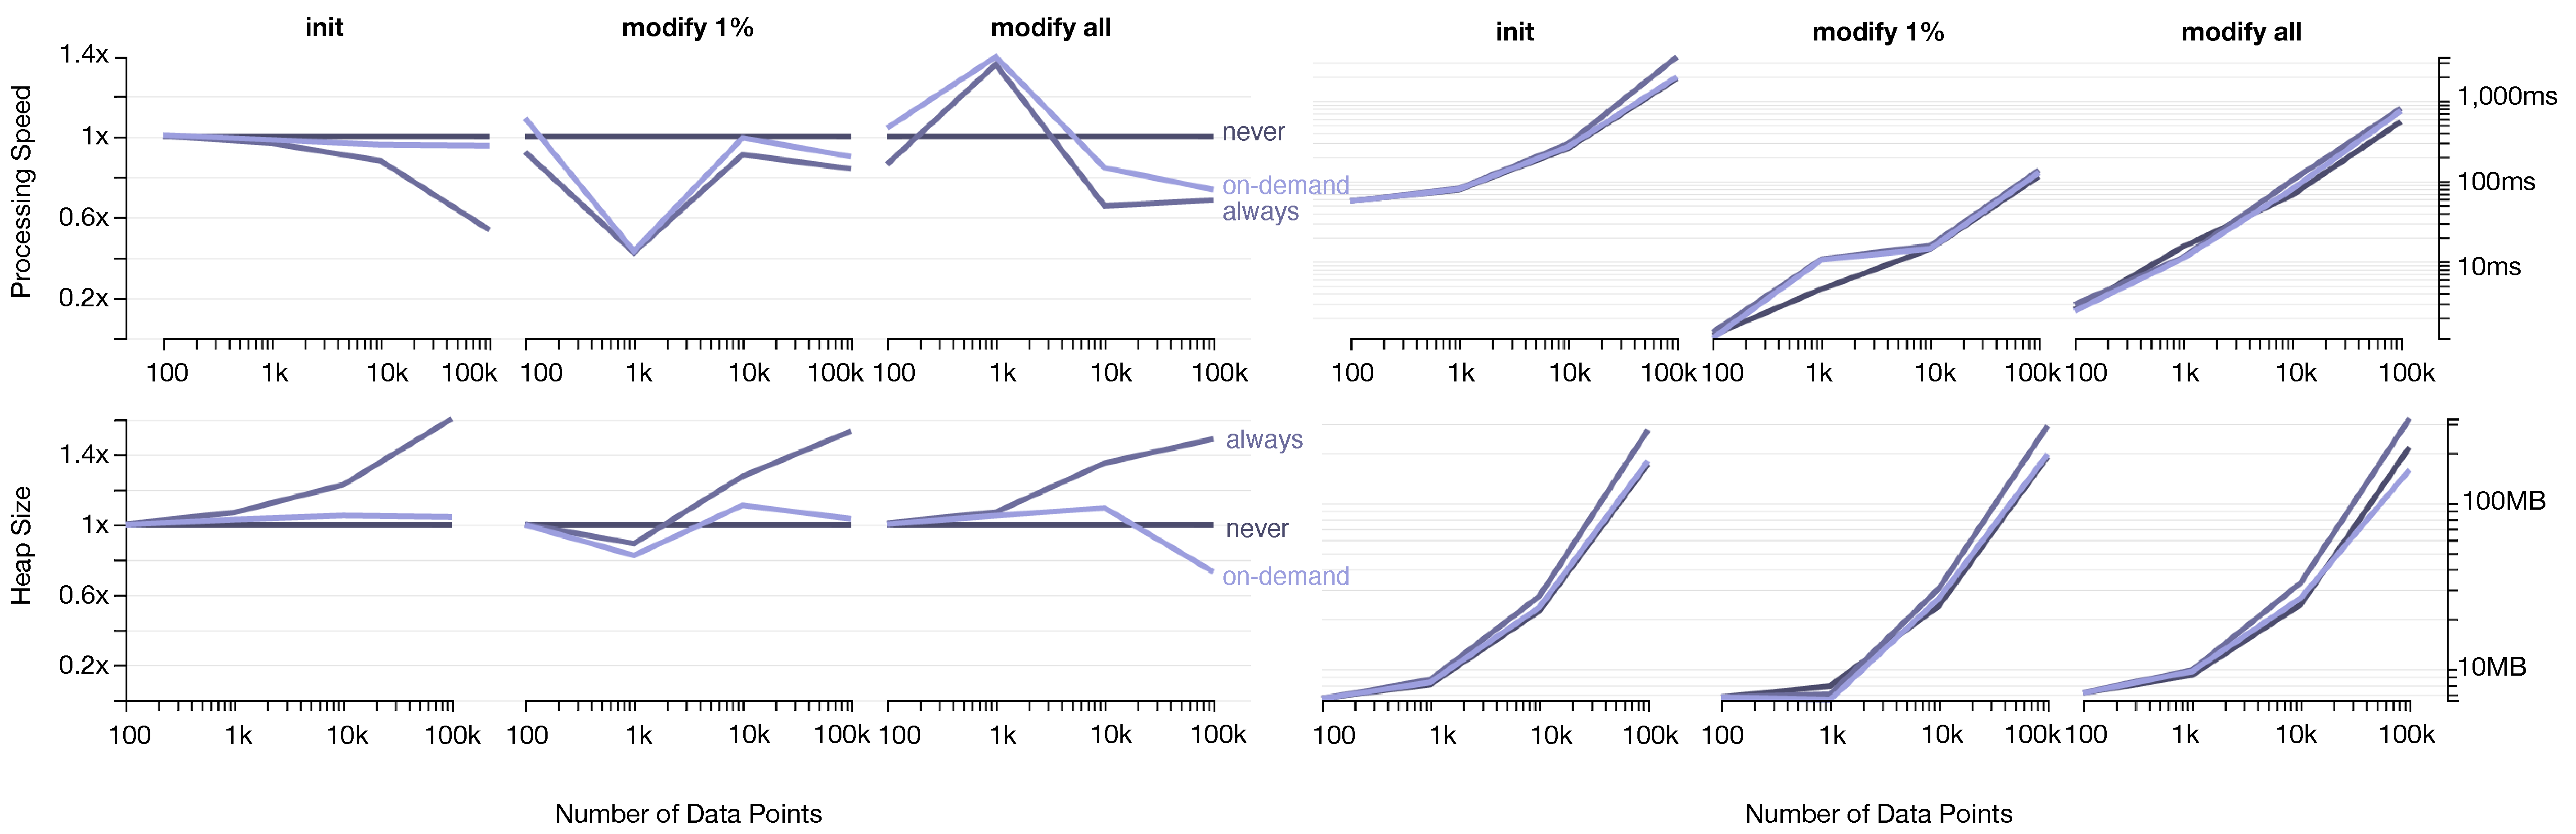
\includegraphics[width=\columnwidth]{prev-lines.pdf}
  \caption{Effects of tuple revision optimizations on average
processing speed (top) and memory footprint (bottom). Left-hand figures show
relative changes using no-tracking as a baseline (closer to 1.0 are better),
and right-hand figures show the absolute values on a log$_{10}$ scale
(lower is better).}
  \label{fig:vg:prev_benchmark}
\end{figure}

Some operators (e.g., statistical aggregates) require both a tuple's current and
previous values. Tracking prior values can affect both running time and memory
consumption. One strategy to minimize this cost is to track tuple revisions only
when necessary. Operators must declare their need for prior values. Then, when
tuples are ingested, their previous values are only tracked if the scheduler
determines that they will flow through an operator that requires revision
tracking.

We ran a benchmark comparing three conditions: always track revisions, never
track revisions, and on-demand tracking. Although the ``never'' condition
produces incorrect results, it provides a lower-bound for performance. We
measured the system's throughput as well as memory allocated when initializing a
scatterplot specification, and after modifying either 1\% or 100\% of input
tuples. The scatterplot features two symbol marks fed by two distinct dataflows,
\texttt{A} and \texttt{B}. Both branches ingest the same set of tuples, and
include operators that derive new attributes. However, \texttt{B} includes
additional aggregation operators that require revision tracking.

The results are shown in Figure~\ref{fig:vg:prev_benchmark}, with the effects of
revision tracking most salient at larger dataset sizes. Always tracking
revisions can require 20-40\% more memory, and can take up to 50\% longer to
initialize a visualization due to object instantiation overhead for storing
previous values. Our on-demand strategy effectively reduces these costs,
requiring only 5-10\% more memory and taking 5\% longer to initialize than the
``never'' condition.

\vspace{-10pt}

\subsection{Pruning Unnecessary Recomputation}
\label{sec:pruning}

\vspace{-7pt}

By centralizing responsibility for operator scheduling and changeset dispatch,
we can aggressively prune unnecessary recomputation. The dataflow graph
scheduler knows the current state of the propagation, and dependency
requirements for each queued operator, allowing us to perform two types of
optimizations:

\begin{enumerate}
  \item \emph{Pruning multiple reflows of the same branch}. As the scheduler
  ensures a topological propagation ordering, a branch can be safely pruned for
  the current propagation if it has already been reflowed.

  \item \emph{Skipping unchanged operators}. Operators identify their
dependencies\,---\,including signals, data fields, and scale functions\,---\,and
changesets maintain a tally of updated dependencies as they flow through the
graph. The scheduler skips evaluation of an individual operator if it is not
responsible for deriving new tuples, or if a changeset contains only modified
tuples and no dependencies have been updated. Downstream operators are still
queued for propagation.
\end{enumerate}

To measure the impact of these optimizations, we created a grouped bar chart
with five data transformation operators: \texttt{Derive(signal1)} $\rightarrow$
\texttt{Fold} $\rightarrow$ \texttt{Derive(signal2)} $\rightarrow$
\texttt{Filter (signal2)} $\rightarrow$ \texttt{Facet}.  We then benchmarked the
effect of four conditions (processing all recomputations, pruning multiple
reflows only, skipping unchanged operators only, and applying both
optimizations) across four tasks (initializing the visualization, updating each
signal in turn, and updating both signals together).

\begin{figure}[b!]
  \centering
  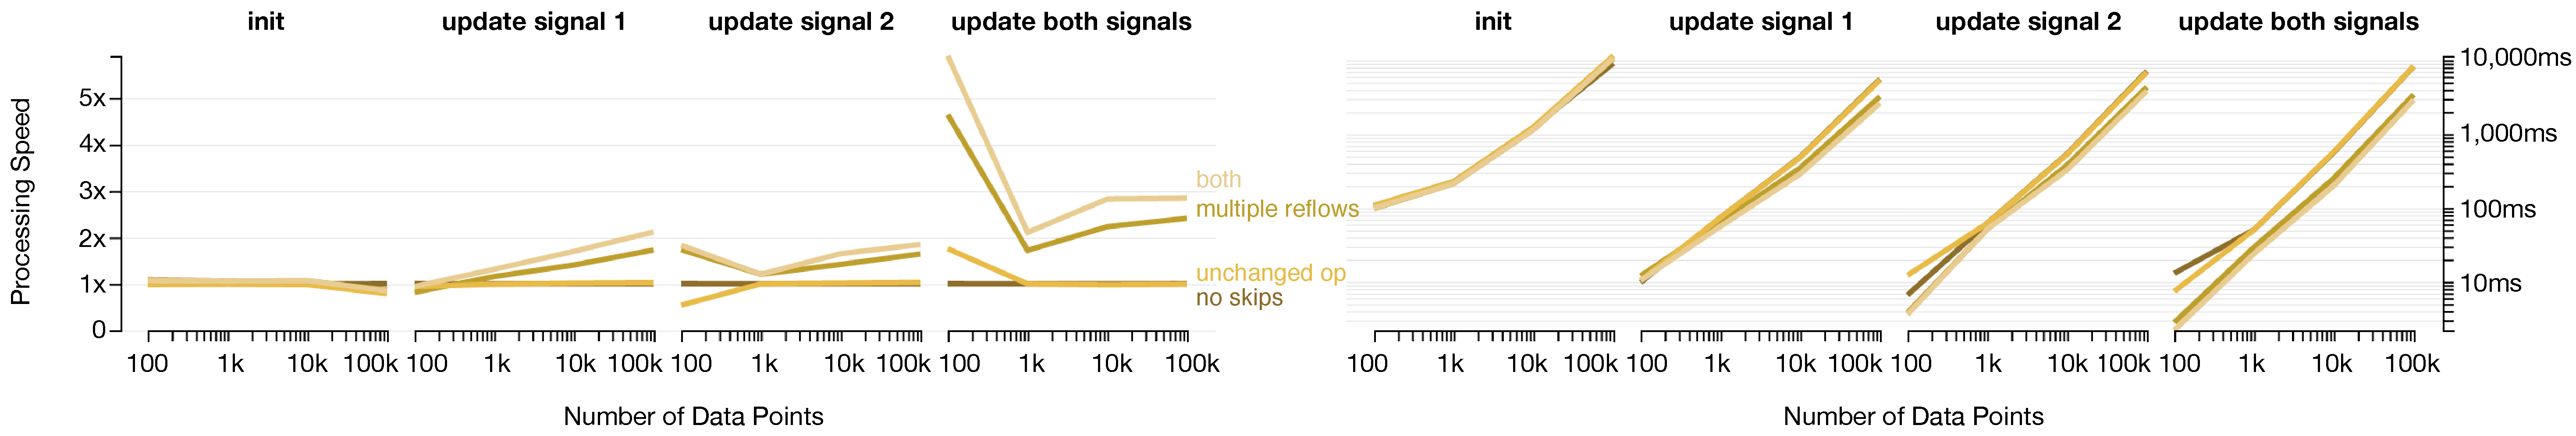
\includegraphics[width=\columnwidth]{skips-lines.pdf}
  \caption{The effects of pruning unnecessary computation on average processing
speed. (a) A relative difference between conditions (higher is better). (b)
Absolute values for time taken, plotted on a log$_{10}$ scale (lower is better).}
  \label{fig:vg:skips_benchmark}
\end{figure}

Results are shown in Figure~\ref{fig:vg:skips_benchmark}. Preventing multiple
reflows is the most effective strategy, increasing throughput 1.4 times on
average. Skipping unchanged operators sees little benefit by itself as, in our
benchmark setup, only the two operators following a fold are skipped when
changing \texttt{signal1}, and only the first derivation operator is skipped
when changing \texttt{signal2}. When the two strategies are combined, however,
we see a 1.6x increase in performance. This result was consistent across
multiple benchmark trials. After careful hand-verification to ensure no
additional nodes were erroneously skipped, we hypothesize that the JavaScript
runtime is able to perform just-in-time optimizations that it is unable to apply
to the other conditions.

\vspace{-10pt}

\subsection{Inlining Sequential Operators}

\vspace{-7pt}

\begin{figure}[b!]
  \centering
  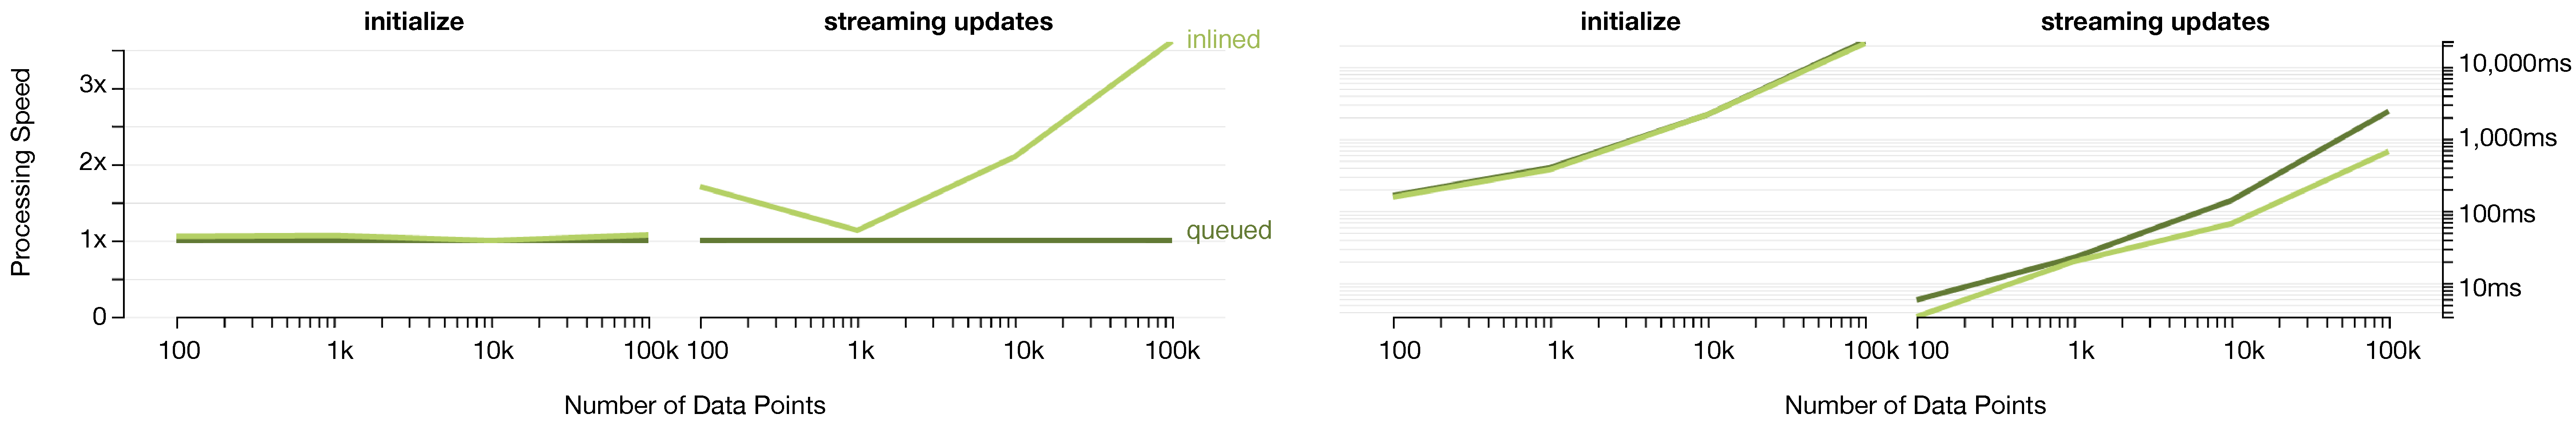
\includegraphics[width=\columnwidth]{inlined-lines.pdf}
  \caption{The effects of inlining sequential operators on average processing
speed. (a) A relative difference between conditions (higher is better). (b)
Absolute values for time taken, plotted on a log$_{10}$ scale (lower is better).}
  \label{fig:vg:inline_benchmark}
\end{figure}

To propagate changesets through the dataflow graph, the scheduler adds operators
to a priority queue, backed by a binary heap sorted in topological order. This
incurs an $O(log N)$ cost for enqueueing and dequeueing operators, which can be
assessed multiple times per operator if the graph is dynamically restructured.
However, branching only occurs when operators register dependencies, and
dependencies are only connected to \texttt{Collector} nodes. As a result, much
of the dataflow graph comprises linear paths. This is particularly true for
scene graph operators, which are grouped into hundreds (or even thousands) of
independent mark build-evaluate-bound branches.

We explore the effect of inline evaluation of linear branches, whereby operators
indicate that their neighbors can be called directly rather than queued for
evaluation. The scheduler remains responsible for propagating the changeset,
and thus can continue to apply the optimizations previously discussed. Although
inline evaluation can be applied in a general fashion by coalescing linear
branches into ``super nodes,'' for simplicity we only evaluate inlining of scene
graph operators here. Mark builders directly call evaluators and bounders, and
group mark builders directly call new child mark builders rather than forming a
temporary connection.

Figure~\ref{fig:vg:inline_benchmark} shows the results of this optimization
applied to a parallel coordinates plot. The plot uses a nested scene graph in
which each line segment is built by a dedicated build-evaluate-bound branch. As
we can see, inlining does not have much impact on the initialization time. This
is unsurprising, as the largest initialization cost is due to unavoidable graph
restructuring. However, inlining improves streaming operations by a 1.9x factor
on average. As streaming updates only propagate down specific branches of the
dataflow graph, inline evaluation results in at least 4 fewer queuing operations
by the scheduler.